% Soubory musí být v kódování, které je nastaveno v příkazu \usepackage[...]{inputenc}

\documentclass[%        Základní nastavení
  %draft,    				  % Testovací překlad
  12pt,       				% Velikost základního písma je 12 bodů
	t,                  % obsah slajdů bude vždy začínat od shora (nebude vertikálně centrovaný)
	aspectratio=1610,   % poměr stran bude 16:10 (všechny projektory v učebnách na Technické 12 Brno),
	                    % další volby jsou 43, 149, 169, 54, 32.
	unicode,						% Záložky a informace budou v kódování unicode
]{beamer}				    	% Dokument třídy 'zpráva', vhodná pro sazbu závěrečných prací s kapitolami
%\usepackage{etex}

\usepackage{graphicx} % Balíček 'graphicx' pro vkládání obrázků
											% Nutné pro vložení logotypů školy a fakulty

\usepackage[          % Balíček 'acronym' pro sazby zkratek a symbolů
	nohyperlinks				% Nebudou tvořeny hypertextové odkazy do seznamu zkratek
]{acronym}						
											% Nutné pro použití prostředí 'acronym' balíčku 'thesis'

%% Balíček hyperref je volán třídou beamer automaticky, proto není třeba následujícího kódu:
%\usepackage[
%	breaklinks=true,		% Hypertextové odkazy mohou obsahovat zalomení řádku
%	hypertexnames=false % Názvy hypertextových odkazů budou tvořeny
%											% nezávisle na názvech TeXu
%]{hyperref}						% Balíček 'hyperref' pro sazbu hypertextových odkazů
%											% Nutné pro použití příkazu 'nastavenipdf' balíčku 'thesis'

\usepackage{cmap} 		% Balíček cmap zajišťuje, že PDF vytvořené `pdflatexem' je
											% plně "prohledávatelné" a "kopírovatelné"

%\usepackage{upgreek}	% Balíček pro sazbu stojatých řeckých písmem
											%% např. stojaté pí: \uppi
											%% např. stojaté mí: \upmu (použitelné třeba v mikrometrech)
											%% pozor, grafická nekompatibilita s fonty typu Computer Modern!

%\usepackage{amsmath} %balíček pro sabu náročnější matematiky

\usepackage{booktabs} % Balíček, který umožňuje v tabulce používat
                      % příkazy \toprule, \midrule, \bottomrule


%%%%%%%%%%%%%%%%%%%%%%%%%%%%%%%%%%%%%%%%%%%%%%%%%%%%%%%%%%%%%%%%%
%%%%%%      Definice informací o dokumentu             %%%%%%%%%%
%%%%%%%%%%%%%%%%%%%%%%%%%%%%%%%%%%%%%%%%%%%%%%%%%%%%%%%%%%%%%%%%%

\input{nastaveni}      % v tomto souboru doplňte údaje o sobě, o názvu práce...
                       % (tento soubor je sdílený s textem práce)
	\usepackage[utf8]		  %	Kódování zdrojových souborů je UTF-8
	{inputenc}					% Balíček pro nastavení kódování zdrojových souborů
\usepackage{fontspec}

%%%%%%%%%%%%%%%%%%%%%%%%%%%%%%%%%%%%%%%%%%%%%%%%%%%%%%%%%%%%%%%%%%%%%%%%

%%%%%%%%%%%%%%%%%%%%%%%%%%%%%%%%%%%%%%%%%%%%%%%%%%%%%%%%%%%%%%%%%%%%%%%%
%%%%%%     Nastavení polí ve Vlastnostech dokumentu PDF      %%%%%%%%%%%
%%%%%%%%%%%%%%%%%%%%%%%%%%%%%%%%%%%%%%%%%%%%%%%%%%%%%%%%%%%%%%%%%%%%%%%%
%% Při vloženém balíčku 'hyperref' lze použít příkaz '\pdfsettings'
\pdfsettings
%  Nastavení polí je možné provést také ručně příkazem:
%\hypersetup{
%  pdftitle={Název studentské práce},    	% Pole 'Document Title'
%  pdfauthor={Autor studenstké práce},   	% Pole 'Author'
%  pdfsubject={Typ práce}, 						  	% Pole 'Subject'
%  pdfkeywords={Klíčová slova}           	% Pole 'Keywords'
%}
\hypersetup{pdfpagemode=FullScreen}       % otevření rovnou v režimu celé obrazovky
%%%%%%%%%%%%%%%%%%%%%%%%%%%%%%%%%%%%%%%%%%%%%%%%%%%%%%%%%%%%%%%%%%%%%%%

\usetheme{VUT} 				% barvy a rozložení prezentace odpovídající VUT FEKT
% alternativně lze použít jiná berevná témata, ale bez záruky. Například: 
%\usetheme{Darmstadt} \usecolortheme{default2}
\logoheader					% vytvoření zkráceného loga VUT FEKT v hlavičce slajdu, nechte odkomentované



\begin{document}

% v případě zakomentování následujícího se zobrazí v pravém dolním rohu slajdů klikatelné navigační symboly 
\disablenavigationsymbols

% titulní snímek, vysazen bez horních, dolních a postranních lišt (volba plain),
% není tak vysazen ani nadpis snímku
\maketitle

%%%%%%%%%%%%%%%%%%%%%%%%%%%%%%%%%%%%%%%%%%%%%%%%%%%%%%%%%%%%%%%%%%%%%%%
% 1. snímek s cíli (zadaním) práce
\begin{frame} 
	% nadpis snímku

% 1. Teoretický průzkum
% 2. Návrh struktruy výsledného systému
% 3. Výběr vhodných metod pro získání parametrů jejich realizace a porovnání

	\frametitle{Cíle práce}
	\begin{block}{Návrh struktruy algoritmu pro generování světelných animací}
		\begin{itemize}
			\item Teoretický průzkum	
			\begin{itemize}
				\item Výzkumů v oblasti Music information retrieval
				\item Možností analýzy parametrů hudební nahrávky
				\item Dostupná řešení extrakce parametrů z hudební nahrávky
			\end{itemize}
			\item Výběr vhodných parametrů
			\item Návrh postupu generování animací na zákaldě vybraných parametrů
		\end{itemize}
	\end{block}
	\begin{block}{Realizace}
		\begin{itemize}
			\item Extrakce parametrů pomocí dostupných metod
			\item Porovnání získaných parametrů a zhodnocení metod
		\end{itemize}
	\end{block}
\end{frame}

%%%%%%%%%%%%%
\begin{frame} 
	\frametitle{Úvod do problematiky}
	\begin{itemize}
		\item Automatické generování animací s dostatečným množstvím času.
	\end{itemize}

	% \begin{block}{Generování světelných animací}
	% 	\begin{itemize}
	% 		\item Z pohledu času
	% 		\begin{itemize}
	% 			\item V minulosti
	% 			\item V reálném čase
	% 		\end{itemize}
	% 		\item Z pohledu způsobu
	% 		\begin{itemize}
	% 			\item navržené člověkem
	% 			\item navržené strojem
	% 		\end{itemize}
	% 	\end{itemize}
	% \end{block}

	\begin{block}{Parametry}
		\begin{itemize}
			\item Jaké parametry využít?
			\item Co tyto parametry ovlivňůjí? 
			\item Jakým způsobem jsou paramety získány?
		\end{itemize}
	\end{block}
\end{frame} 

\begin{frame}
	\frametitle{Výběr}
	Vybrané parametry hudební nahrávky pro generování světelných animací.
	\begin{columns}[T]
		\begin{column}{0.3\textwidth}		% první sloupec
			\begin{itemize}
				\item Detekce dob
				\item Chroma vektory
				\item Tempo
				\item Efektivní hodnota 
				\item Segmenty
				\item Žánr
				\item Nálada
			\end{itemize}
		\end{column}
		\begin{column}{0.7\textwidth}		
			% \includegraphics[width = 0.6\columnwidth]{obrazky/Prez_parametry.pdf}
		\end{column}
		
	\end{columns}
\end{frame}

\begin{frame}
	\frametitle{Využití}
	\begin{block}{Výběr datasetu}
	\end{block}
	\vspace{1cm}

	\includegraphics[width = 1\columnwidth]{obrazky/Dataset_selection_diagram.pdf}

\end{frame}

\begin{frame}
	\frametitle{Využití}
	\begin{block}{Umístění bloků animací v čase}
		\begin{itemize}
			\item Začátek dle dob
			\item Délka dle tempa a efektivní hodnoty
			\item Konec dle délky animace zaorkouhlené na nejbližší dobu
		\end{itemize}
	\end{block}
	\begin{block}{Výběr bloku animace}
		\begin{itemize}
			\item Výběr na základě efektivní hodnoty v čase bloku animace
		\end{itemize}
	\end{block}

	\begin{block}{Barevná paleta}
		\begin{itemize}
			\item Vytvoření palety barev z analýzy chromavektorů nahrávky
			\item Určení znějících tónů v čase bloku animace z chromavektorů
			\item Přiřazení bloku animace barvy dle tónů a palety barev
		\end{itemize}
	\end{block}
\end{frame}

% \begin{frame}
% 	\frametitle{}
% 	\includegraphics[width = 0.4\columnwidth]{obrazky/Logical_structure_diagram.pdf}
% \end{frame}

\begin{frame}
	\frametitle{Extrakce}
	\begin{block}{Využité knihovny}
		\begin{itemize}
			\item Librosa
				\begin{itemize}
					\item Detekce dob a tempa
					\item Analýza chromavektorů
					\item Výpočet efektivní hodnoty
				\end{itemize}
			\item Madmom
				\begin{itemize}
					\item Detekce dob a tempa
					\item Analýza chromavektorů
				\end{itemize}
			\item Aubio
				\begin{itemize}
					\item Detekce dob a tempa
				\end{itemize}
			\item Mir\_eval
				\begin{itemize}
					\item Výpočet Cemgil skóré pro porovnání detekce dob
				\end{itemize}
		\end{itemize}
	\end{block}
	% Použité knihovny metody 
	% Hodnocení metod a posání výsledků
\end{frame}

\begin{frame}
	\frametitle{}
	\centering
	\includegraphics[width = 1\columnwidth]{obrazky/Beat_track_presentation.eps}
\end{frame}

\begin{frame}
	\frametitle{}
	\centering
	\includegraphics[width = 0.75\columnwidth]{obrazky/Beat_tracking_time_and_cemgil_graphs.eps}
\end{frame}

\begin{frame}
	\frametitle{}
	\centering
	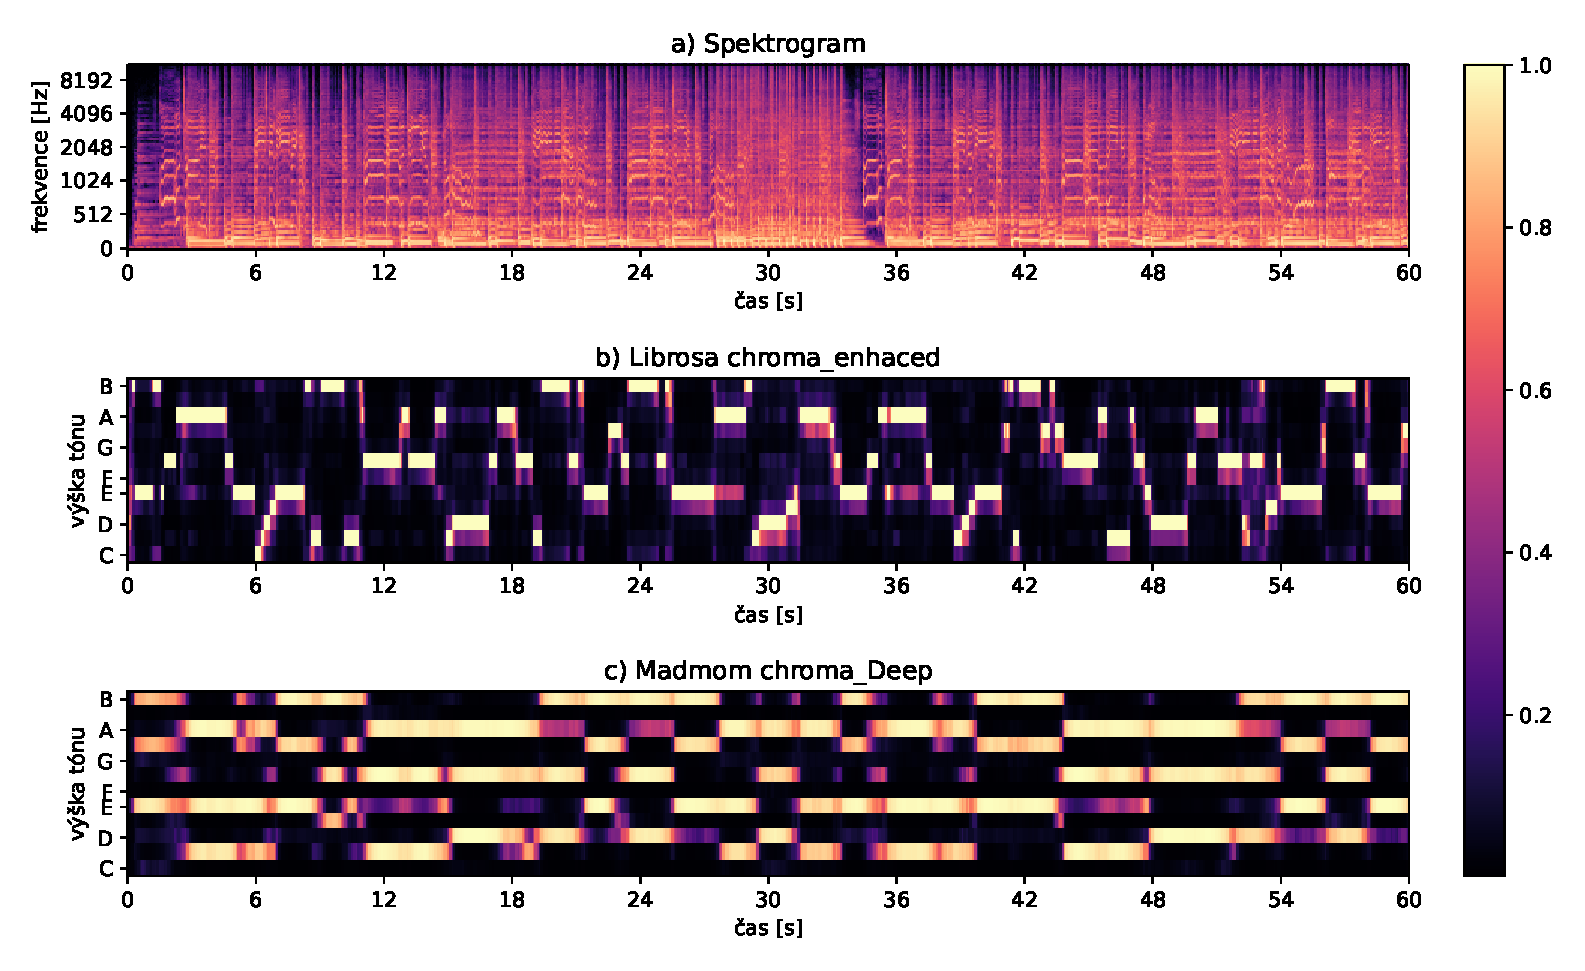
\includegraphics[width = 1\columnwidth]{obrazky/Chromavector_presentation.eps}
\end{frame}

\begin{frame}
	\frametitle{}
	\centering
	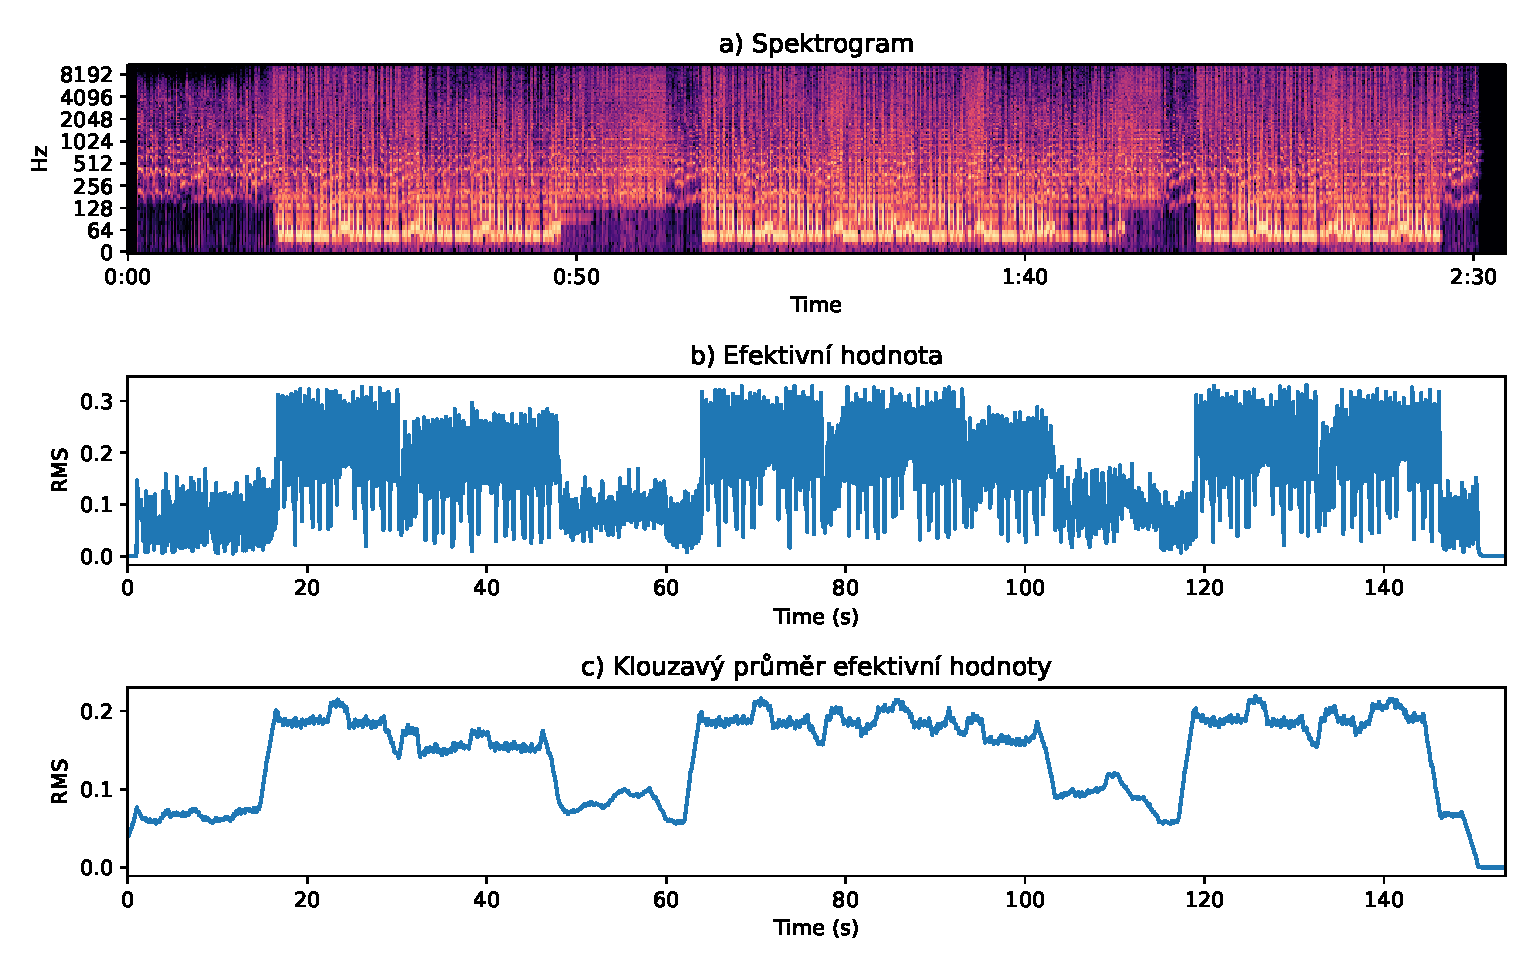
\includegraphics[width = 1\columnwidth]{obrazky/Belly_dancer_RMS.eps}
\end{frame}


% Shrnutí (přídána obálka síly nástupu)

\begin{frame} 
	\frametitle{Závěr}
	\begin{block}{Splnění cílů}
		\begin{itemize}
			\item Teoretický průzkum
			\item Návrh struktury výsledného algoritmu
			\item Extrakce a porovnání parametrů
		\end{itemize}
	\end{block}
	\begin{block}{Diplomová práce a návrhy na zlepšení}
		\begin{itemize}
			\item Segmentace nahrávky
			\item Rozpoznávání žánrů
			\item Využití obálky síly nástupů
			\item Realizace a optimalizace funkčního systému pro generování animací
		\end{itemize}
	\end{block}
\end{frame}

% podekovani
\begin{frame}[c] 
% bez nadpisu snímku
	\frametitle{\mbox{ }}
	\begin{center}
		{\Huge Děkuji za pozornost!}
	\end{center}
\end{frame}

\end{document}
